\documentclass{exam}
\usepackage{../../mypackages}
\usepackage{../../macros}

\title{Correction - Interro N°2 - Atome et Réactions Chimiques}
\author{N. Bancel}
\date{Novembre 2024}

\begin{document}

\textbf{Collège Lycée Suger}
\hfill
\textbf{Physique-Chimie} \\

\textbf{Année 2024-2025}
\hfill
\textbf{3ème Cambridge International} \par

{\let\newpage\relax\maketitle}

\begin{center}
\textbf{\textcolor{red}{Durée : 45 minutes. La calculatrice n'est pas autorisée}} \\
\textbf{\textcolor{red}{Une réponse donnée sans justification sera considérée comme fausse.}} \\
Cette interrogation contient \numquestions\ questions, sur \numpages\ pages et est notée sur 10. 
\end{center}

\begin{tcolorbox}[colback=green!10!white, colframe=green!75!black, title=A retravailler et à assimiler à tout prix]
  \begin{itemize}[noitemsep]
    \item Connaître sur le bout des doigts la signification de A, de Z, et de X
    \item Comprendre pourquoi l'atome est électriquement neutre et la constitution d'un atome (Nombre de protons = Nombre d'électrons. Nombre de nucléons = Nombre de neutrons + Nombre de protons)
    \item Equilibrer une équation chimique : on ne PEUT PAS modifier la structure d'une molécule pour équilibrer une équation. On ne peut que MULTIPLIER la quantité de cette molécule.
    \item Comprendre dans une phrase quels sont les réactifs et les produits, en identifiant les verbes (brûle, réagit avec... : réactifs) (produit, génère, se transforme en : produits)
    \item Savoir poser un ratio, une division.
    \item Comprendre le concept de conservation de la masse
  \end{itemize}
\end{tcolorbox}

\section*{Partie 1 : Structure de l'Atome et Propriétés (5 points)}

\begin{questions}
  \question[1] Donnez la signification de $A$, $X$, et $Z$ dans la notation symbolique d'un atome.

  \begin{figure}[H]
    \centering
    
\includegraphics[width=0.2\linewidth]{interro2_01.jpg}
    \caption{Structure simplifiée d'un atome}
\end{figure} 

  \textbf{\textcolor{blue}{Réponse :}} \\
  Dans la notation symbolique d'un atome, $X$ représente le symbole chimique de l'élément, $A$ est le nombre de masse (il représente le nombre de nucléons = nombre de protons + nombre de neutrons) dans le noyau, et $Z$ est le numéro atomique (nombre de protons). Par exemple, pour l'atome de carbone ${}^{12}_{6}\text{C}$, $A = 12$ et $Z = 6$.

  \question[1.5] Complétez la figure ci-dessous en remplissant les cases manquantes.

  \begin{figure}[H]
    \centering
    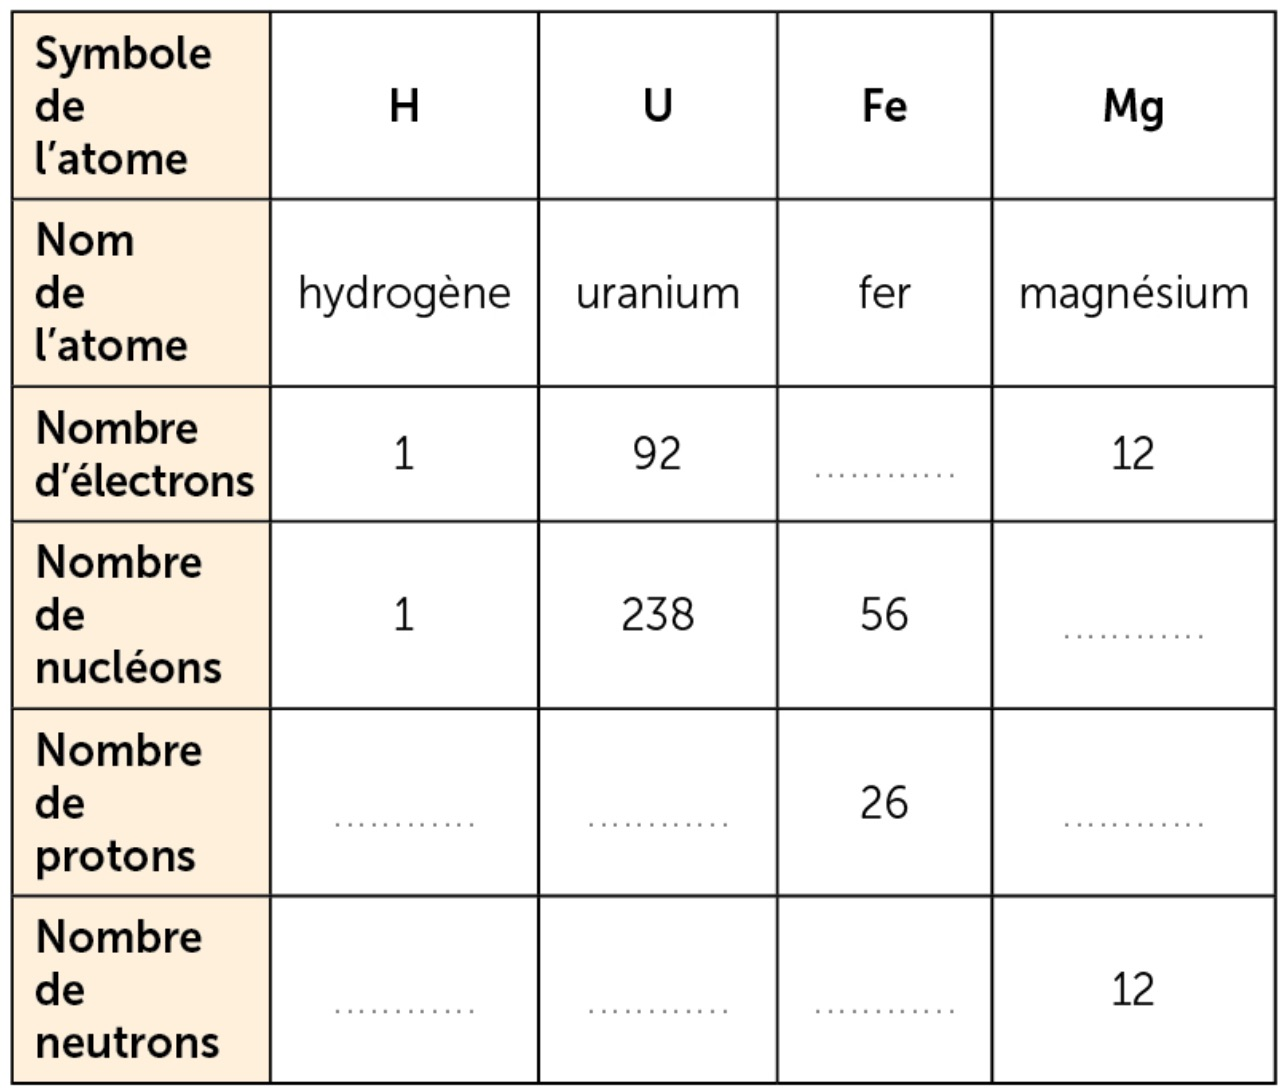
\includegraphics[width=0.6\linewidth]{interro2_02.jpg}
    \caption{Composants de l'atome}
\end{figure} 

  \textbf{\textcolor{blue}{Réponse :}} \\
  
  Pour remplir ce tableau, nous avons utilisé les règles suivantes :

\begin{itemize}
    \item \textbf{Nombre de protons} : Le nombre de protons est égal au nombre d'électrons dans un atome, car les charges positives (protons) et les charges négatives (électrons) s'équilibrent (L'atome étant électriquement neutre)
    \item \textbf{Nombre de nucléons} : Par définition, les nucléons correspondent à l'ensemble des particules du noyau, et incluent donc les protons et les neutrons. Donc 
    \[
    \text{Nombre de nucléons} = \text{Nombre de neutrons} + \text{Nombre de protons}
    \]
    \item \textbf{Nombre de neutrons} : Le nombre de neutrons se calcule en soustrayant le nombre de protons du nombre de nucléons (qui correspond au nombre de masse de l'atome). La formule est donc :
    \[
    \text{Nombre de neutrons} = \text{Nombre de nucléons} - \text{Nombre de protons}
    \]
\end{itemize}

Voici le détail pour chaque atome :

\begin{itemize}
  \item \textbf{Hydrogène (H)} : 
  \begin{itemize}
      \item Nombre de protons = 1, car nombre d'électrons = 1.
      \item Nombre de neutrons = Nombre de nucléons - Nombre de protons = 1 - 1 = 0.
  \end{itemize}

    \item \textbf{Uranium (U)} : 
    \begin{itemize}
        \item Nombre protons = 92, car nombre d'électrons = 92.
        \item Nombre de neutrons = Nombre de nucléons - Nombre de protons = 238 - 92 = 146.
    \end{itemize}
    
    \item \textbf{Fer (Fe)} :
    \begin{itemize}
        \item Nombre d'électrons = 26, car nombre de protons = 26.
        \item Nombre de neutrons = Nombre de nucléons - Nombre de protons = 56 - 26 = 30.
    \end{itemize}
    
    \item \textbf{Magnésium (Mg)} :
    \begin{itemize}
        \item Nombre protons = 12, car nombre d'électrons = 12.
        \item Nombre de nucléons = Nombre de neutrons + Nombre de protons = 12 - 12 = 24.
    \end{itemize}
\end{itemize}

\begin{table}[H]
  \centering
  \begin{tabularx}{\textwidth}{|X|c|c|c|c|}
  \hline
  \textbf{Symbole de l’atome} & \textbf{H} & \textbf{U} & \textbf{Fe} & \textbf{Mg} \\
  \hline
  \textbf{Nom de l’atome} & hydrogène & uranium & fer & magnésium \\
  \hline
  \textbf{Nombre d’électrons} & 1 & 92 & 26 & 12 \\
  \hline
  \textbf{Nombre de nucléons} & 1 & 238 & 56 & 24 \\
  \hline
  \textbf{Nombre de protons} & 1 & 92 & 26 & 12 \\
  \hline
  \textbf{Nombre de neutrons} & 0 & 146 & 30 & 12 \\
  \hline
  \end{tabularx}
  \end{table}


  \question[0.5] Expliquez pourquoi un atome est neutre électriquement.

  \textbf{\textcolor{blue}{Réponse :}} \\
  Un atome est neutre électriquement car le nombre de charges positives (protons) est égal au nombre de charges négatives (électrons). Les charges se compensent donc, rendant l’atome neutre.

  \question[1.5] Basé sur les informations ci-dessous, de combien de fois la masse d’un nucléon est-elle supérieure à celle d’un électron ? 

  \begin{center}
    \begin{tabular}{SS}
      \toprule
      {Constituant} & {Masse (en \si{kg})} \\
      \midrule
      {Electron} & {\(9.1 \times 10^{-31}\)} \\
      {Nucléon (Proton et Neutron)} & {\(1.7 \times 10^{-27}\)} \\
      \bottomrule
    \end{tabular}
  \end{center}
    

  \textbf{\textcolor{blue}{Réponse :}} \\
  \textbf{\textcolor{red}{Pour trouver combien de fois A est plus grand que B, on calcule le rapport de $\frac{A}{B}$ (on divise A par B, et on donne le résultat). Si vous mesurez 1.5m et que vous surfez une vague de 4.5m, la vague est 3 fois plus grande que vous. Parce que vous avez calculé $\frac{4.5}{1.5} = 3$}} \\
  \vspace{1em}
  Trouver de combien de fois la masse d'un nucléon $m_n$ est plus grande que la masse d'un électron $m_e$, cela revient à calculer la valeur du rapport : $\frac{m_n}{m_e}$
\[
m_e = 9.1 \times 10^{-31} \, \si{kg}, \quad m_n = 1.7 \times 10^{-27} \, \si{kg}
\]

Le ratio \(\frac{m_n}{m_e}\) est donc :
\[
\frac{m_n}{m_e} = \frac{1.7 \times 10^{-27}}{9.1 \times 10^{-31}}
\]

Utilisons les propriétés des puissances de 10. Lorsqu'on divise deux puissances de 10, on soustrait leurs exposants :
\[
\frac{10^{-27}}{10^{-31}} = 10^{(-27 - (-31))} = 10^{4}
\]

Le ratio des coefficients est calculé séparément :
\[
\frac{1.7}{9.1} \approx 0.187
\]

Le produit final est donc :
\[
\frac{m_n}{m_e} = 0.187 \times 10^4 = 1.87 \times 10^3
\]

Ce résultat montre que la masse d'un nucléon est environ \(1.87 \times 10^3\) fois plus grande que celle d'un électron. Cependant, pour simplifier l'ordre de grandeur, on arrondit souvent ce ratio à 2000 :
\[
\frac{m_n}{m_e} \approx 2000
\]

\[
m_n \approx 2000 \times {m_e}
\]
  
  La masse d'un nucléon est environ 2000 fois supérieure à celle d'un électron.

  \question[0.5] Expliquer la différence entre un atome et une molécule, et donnez un exemple de chaque.

  \textbf{\textcolor{blue}{Réponse :}} \\
  Un atome est la plus petite unité d’un élément chimique, comme un atome d'hydrogène (\ce{H}). Une molécule est un ensemble d’atomes liés entre eux, comme une molécule d'eau (\ce{H2O}).

\end{questions}

\section*{Partie 2 : Réactions chimiques (5 points)}

\begin{questions}

  \question[0.75] Donnez les formules des molécules suivantes :
  \begin{itemize}[noitemsep]
    \item Dioxygène : \ce{O2}
    \item Dioxyde de carbone : \ce{CO2}
    \item Eau : \ce{H2O}
  \end{itemize}

  \question[1] La paille de fer (\ce{Fe}) brûle facilement dans l'air (au contact du dioxygène \ce{O2}). Il se forme alors de petites boules d'oxyde magnétique de fer, de formule \ce{Fe3O4}. 
  \begin{parts}
    \part[0.25] Quelle est la constitution en atomes de l'oxyde magnétique de fer ? Préciser le nom et le nombre de chaque type d'atomes. \\
    \textbf{\textcolor{blue}{Réponse :}} \\
    La molécule de \ce{Fe3O4} est constituée de 3 atomes de fer (Fe) et 4 atomes d’oxygène (O).

    \part[0.25] Écrire en toutes lettres la réaction chimique traduisant la transformation entre le fer et le dioxygène de l'air. \\
    \textbf{\textcolor{blue}{Réponse :}} \\
    \textbf{Dans un énoncé de ce type : XX brûle / réagit avec YYY pour former ZZZ. Faire bien attention aux verbes. Tout ce qui est du champ lexical de la création, la formation correspond aux produits. Tout ce qui est du champ lexical de la réaction, de la combustion, de la brûlure, de la dillution correspond aux réactifs}
    Fer + Dioxygène \(\rightarrow\) Oxyde magnétique de fer.

    \part[0.5] Écrire et équilibrer l'équation chimique qui a lieu.
    \textbf{\textcolor{blue}{Réponse :}} \\
    L'équation chimique équilibrée est : \ce{3 Fe + 2 O2 -> Fe3O4}. \\
    Il y a ainsi 3 atomes de Fe à gauche et à droite \\
    Et il y a 4 atomes d'oxygène à gauche et à droite
  \end{parts}
  
  \question[1] Adam réalise l'expérience schématisée ci-dessous.

  \begin{figure}[H]
      \centering
      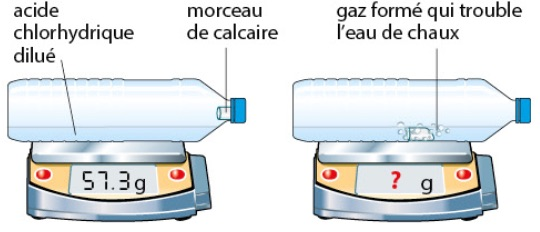
\includegraphics[width=0.6\linewidth]{interro2_03.jpg}
      \caption{Expérience de transformation chimique}
  \end{figure} 

  \begin{parts}
    \part[0.25] Quels sont les réactifs ? Quels sont les produits ?
    \textbf{\textcolor{blue}{Réponse :}} \\
    Les réactifs sont l'acide chlorydrique dilué et le calcaire. \\ 
    Le produit est un gaz qui trouble l'eau de chaux : d'après le cours, on sait que c'est du dioxyde de carbone 

    \part[0.25] Quelle est la masse de ces réactifs ?
    \textbf{\textcolor{blue}{Réponse :}} \\
    La masse totale des réactifs est égale à la masse mesurée initialement sur la balance de gauche. Elle vaut 57.3g. 

    \part[0.5] Qu'indique la balance de droite ? Pourquoi ?
    \textbf{\textcolor{blue}{Réponse :}} \\
    La balance de droite montre que la masse reste la même après la réaction, par la loi de conservation de la masse.
    Elle indique donc 57.3g
  \end{parts}

  \question[1.5] Les équations chimiques ci-dessous sont-elles équilibrées ? Justifier pourquoi. Si elles ne le sont pas, les équilibrer.

  \textbf{\textcolor{red}{Quand on équilibre une équation, on ne peut pas toucher à la formule de la molécule. Si on a du \ce{H2O}, c'est de l'eau, on ne peut pas transformer ça en \ce{H204} pour équilibrer. On doit garder la structure de la molécule, mais on peut en revanche multiplier sa quantité. Le nombre / le coefficient se situe donc DEVANT la molécule}}
  \begin{parts}
    \part[0.5] \ce{H2O -> H2 + O2} \\
    \textbf{\textcolor{blue}{Réponse :}} \\
    Cette équation n'est pas équilibrée car il y a 2 atomes d'oxygène à droite et seulement 1 à gauche. L'équation équilibrée est : \ce{2 H2O -> 2 H2 + O2}.

    \part[0.5] \ce{C + O2 -> CO} \\
    \textbf{\textcolor{blue}{Réponse :}} \\
    Cette équation n'est pas équilibrée car il manque un atome d'oxygène. L'équation équilibrée est : \ce{2 C + O2 -> 2 CO}.

    \part[0.5] \ce{CH4 + O2 -> CO2 + H2O} \\
    \textbf{\textcolor{blue}{Réponse :}} \\
    Cette équation n'est pas équilibrée car il y a 2 atomes d'oxygène à gauche et 3 à droite. L'équation équilibrée est : \ce{CH4 + 2 O2 -> CO2 + 2 H2O}.
  \end{parts}

  \question[0.75] Quelle est la formule de la réaction chimique complète entre le dihydrogène et le dioxygène ? \\
  \textbf{\textcolor{blue}{Réponse :}} \\
  L'atome de couleur rouge correspond à l'atome d'oxygène. L'atome de couleur blanche correspond à l'atome d'hydrogène.
  Les 2 atomes rouges (oxygène) sont collés donc ils forment une molécule, composé de 2 atomes d'oxygène. C'est du \ce{O2}
  Les 2 atomes blancs (hydrogène) sont collés donc ils forment une molécule, composé de 2 atomes d'hydrogène. C'est du \ce{H2}. Il y a 2 molécules de ce type donc la formule contiendra \ce{2H2}
  Côté produits, il y a 2 molécules formées. Chacune composée de 1 atome d'oxygène (rouge) et de 2 atomes d'hydrogène (blancs). On a donc du \ce{2 H2O} côté produits.
  La réaction chimique est la suivante : \\
  \ce{2 H2 + O2 -> 2 H2O}.
  Elle est équilibrée car on trouve le même nombre d'atomes de part et d'autre de l'équation. Il y a conservation de la masse
  
\end{questions}

\end{document}
